\section{Implementação do Algoritmo Sunny}
\label{sec:7.1}

No Sunny, a execução do algoritmo genético ocorre no serviço responsável pela geração da grade horária. Esse serviço recebe uma requisição contendo os dados acadêmicos necessários ao processo de alocação, como turmas, matrizes curriculares, disponibilidades docentes e vínculos entre usuários e disciplinas. A partir dessas informações, o algoritmo constrói uma estrutura de contexto denominada EvolutionContext, utilizada para organizar os parâmetros, os mapas auxiliares e os caches necessários durante uma execução específica.

Essa organização é importante porque o algoritmo genético realiza avaliações repetidas. A cada geração, vários indivíduos são avaliados, selecionados, recombinados e modificados. Caso todas essas verificações fossem feitas diretamente sobre as listas originais da requisição, o custo computacional tenderia a ser maior e a implementação ficaria menos eficiente. Por esse motivo, o Sunny cria estruturas de acesso rápido, como mapas de disponibilidades, matrizes, turmas, professores habilitados por disciplina, disponibilidades por turno, turno obrigatório de cada matriz, usuário associado a cada disponibilidade e dia da semana correspondente a cada horário.

Essa etapa pode ser compreendida como uma adaptação prática do conceito de ambiente apresentado no Capítulo 3. Na biologia, o ambiente é o espaço em que os organismos competem, sobrevivem e são selecionados. No algoritmo genético, esse ambiente é representado pelo próprio problema e por suas restrições. No caso do Sunny, ele é formado pelas regras de alocação acadêmica: uma matriz curricular precisa ser associada a uma disponibilidade compatível, o professor precisa estar habilitado para a disciplina, o turno da disponibilidade deve corresponder ao turno da turma e conflitos de horário precisam ser evitados.

A implementação estabelece que os valores utilizados pelo microsserviço sejam definidos por meio de parâmetros armazenados na tabela de configuração do sistema principal, permitindo ao administrador personalizar o comportamento do algoritmo conforme as necessidades institucionais. Atualmente, o banco de dados possui valores padrão definidos a partir de um extenso processo de testes de desempenho, os quais serão detalhados em seção específica, em que diferentes configurações foram avaliadas com o objetivo de identificar aquelas que apresentavam melhor performance, menor incidência de erros, menor tempo de execução e menor consumo de recursos durante a geração das grades.

A forma como uma solução é representada é uma das decisões mais relevantes em um algoritmo genético. No Sunny, cada gene é composto por dois elementos principais: matrizId e disponibilidadeId. O campo matrizId identifica a demanda acadêmica que precisa ser alocada, enquanto o campo disponibilidadeId indica a disponibilidade escolhida para essa demanda. O cromossomo, por sua vez, é formado por uma lista desses genes e representa uma grade horária candidata completa. Essa codificação traduz o problema real para uma estrutura que pode ser manipulada computacionalmente. No domínio acadêmico, o sistema precisa montar uma grade de aulas. No domínio genético, o algoritmo trabalha com listas de pares entre matrizes e disponibilidades. Quando uma demanda não pode ser alocada de maneira compatível, o Sunny utiliza o valor ID\_NAO\_ALOCADO = 0.

A população inicial do Sunny é formada por cromossomos gerados a partir dos dados recebidos na requisição. Essa geração não ocorre de forma totalmente aleatória. Para cada matriz curricular, o Sunny verifica inicialmente o turno obrigatório associado à turma, busca as disponibilidades compatíveis com esse turno, identifica os professores habilitados para a disciplina correspondente e filtra as disponibilidades pertencentes a esses professores. Somente após essa etapa de filtragem o algoritmo escolhe aleatoriamente uma disponibilidade entre as alternativas consideradas válidas. Essa abordagem pode ser classificada como uma inicialização aleatória guiada por restrições, aproximando-se da ideia de codificação restritiva discutida por \citeonline{michalewicz1996}.

A função \textit{fitness} é o mecanismo utilizado pelo Sunny para medir a qualidade de cada cromossomo. No Sunny, a avaliação começa com uma pontuação base proporcional ao número de genes do cromossomo, com valor padrão de 10 pontos por gene. Em seguida, a função percorre os genes e aplica penalidades ou bônus conforme as condições encontradas. Quando um gene está marcado como não alocado, o indivíduo recebe uma penalidade padrão de 10.000 pontos. A mesma penalidade de 10.000 pontos é aplicada quando os dados necessários à avaliação estão incompletos ou inválidos, como ausência de professor, dia ou turno associado à alocação. O Sunny também verifica conflitos de professor por meio de uma chave composta por usuário, dia e turno. Se mais de uma matriz for associada ao mesmo professor no mesmo período, o algoritmo identifica uma colisão e aplica 10.000 pontos de penalidade para cada conflito excedente. A função \textit{fitness} também aplica um bônus de diversidade associado à quantidade de matrizes atribuídas a um professor, com valor padrão de 5 pontos para cada matriz adicional, de modo que ele atua como critério secundário sem se sobrepor à prioridade de reduzir alocações inválidas.

Após a avaliação, o Sunny ordena os indivíduos e aplica duas estratégias: elitismo e seleção por torneio. O elitismo preserva diretamente uma parcela dos melhores indivíduos para a geração seguinte, evitando que boas soluções sejam perdidas por alterações dos operadores evolutivos. A seleção dos pais é realizada por torneio, no qual o algoritmo escolhe aleatoriamente um grupo de indivíduos e seleciona o melhor entre eles, criando pressão seletiva com grau de aleatoriedade que preserva a diversidade populacional.

O \textit{crossover} do Sunny utiliza uma estratégia próxima do \textit{crossover} uniforme, em que o método percorre cada posição do cromossomo e decide aleatoriamente se o gene daquela posição será herdado do primeiro ou do segundo pai. A mutação é aplicada gene a gene: para cada gene, o algoritmo sorteia uma probabilidade e, caso seja inferior à taxa configurada, substitui a disponibilidade associada àquela matriz. Quando a mutação ocorre, o Sunny não escolhe uma nova disponibilidade de forma irrestrita; o algoritmo consulta novamente o turno obrigatório e filtra os professores habilitados antes de escolher aleatoriamente uma alternativa válida.

Após a recombinação e a mutação, o Sunny executa um mecanismo de reparo parcial que identifica situações em que uma mesma turma possui mais de uma alocação no mesmo dia e turno. Quando isso ocorre, o algoritmo preserva a primeira ocorrência e marca as demais como não alocadas. O Sunny não realiza reparo por realocação; o que existe é um reparo parcial por invalidação de alocações conflitantes. Essa abordagem combina duas estratégias de tratamento de restrições: reparo e penalização.

Ao final da execução, o melhor cromossomo encontrado é decodificado em uma lista de alocações de grade. Na decodificação, cada gene é transformado em uma estrutura de alocação contendo turma, matriz, disciplina, disponibilidade, professor e status. O Sunny calcula então as métricas finais, que contabilizam disciplinas não alocadas, inconsistências de turno e conflitos de horário de professor. O ciclo evolutivo é executado até atingir o número máximo de gerações definido nos parâmetros, registrando ao longo da execução a geração em que uma solução sem erros é encontrada, sem que isso interrompa o laço evolutivo.


\begin{figure}[H]
\centering
\caption{Fluxo de execução do algoritmo genético Sunny}
\label{fig:fluxo-sunny}

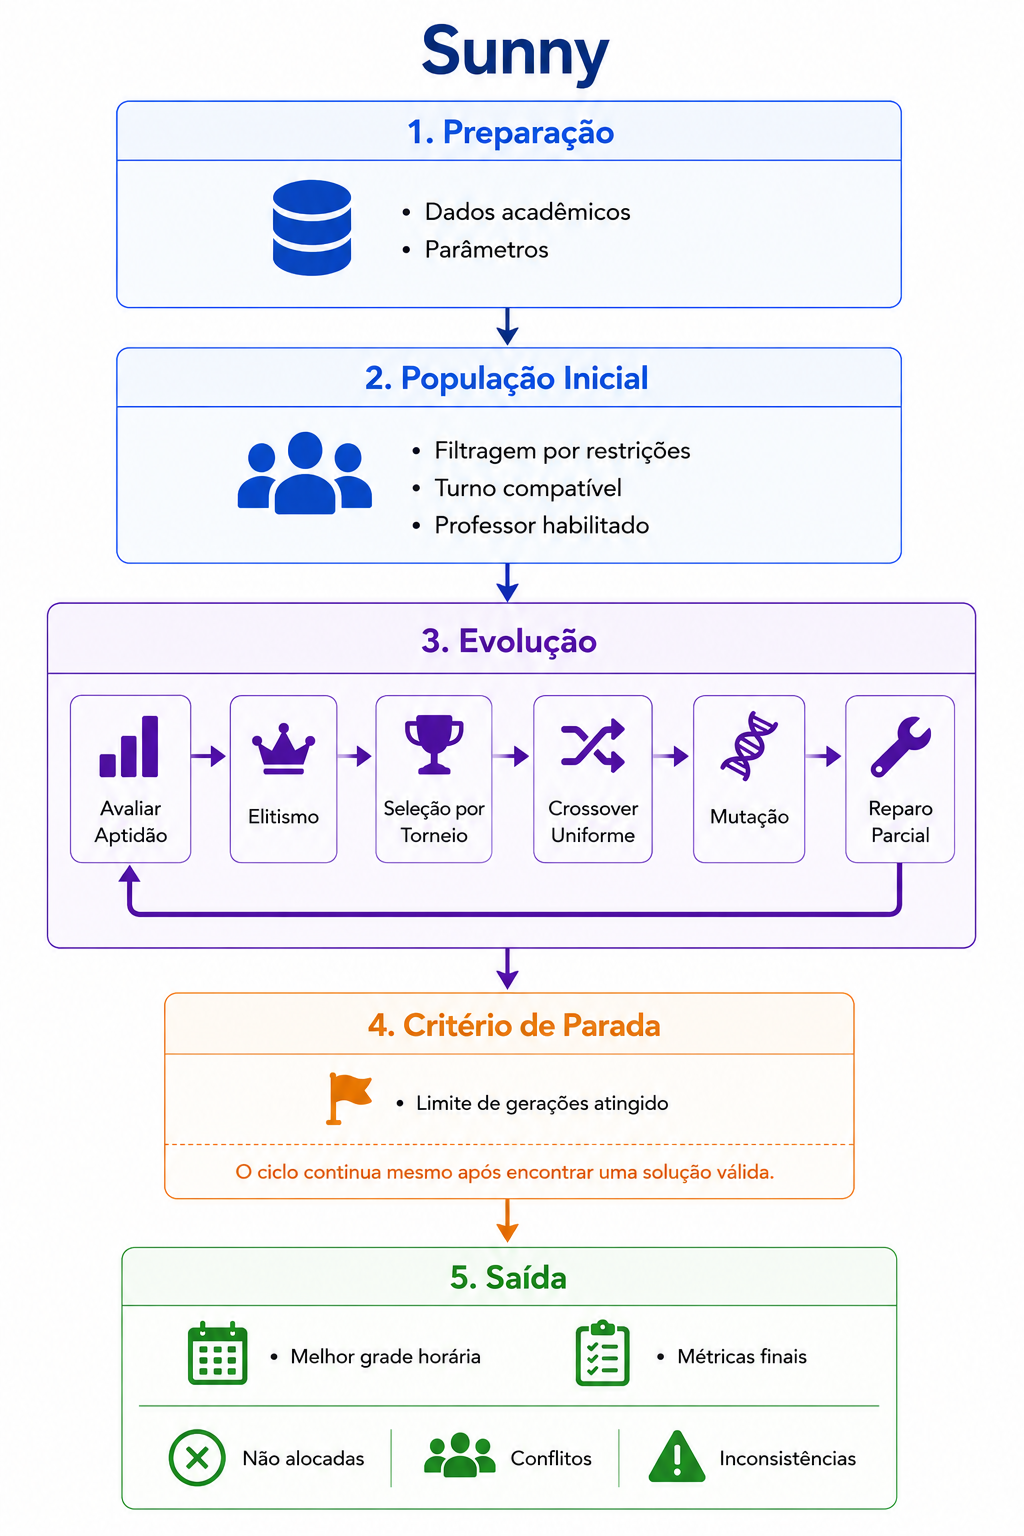
\includegraphics[width=0.85\textwidth]{figuras/Figura_15_ilustracaoFluxoSunny.png}

\vspace{0.2cm}
\fonteautores
\end{figure}
